\documentclass[tikz,border=10pt]{standalone}
\usepackage{amsmath}
\usepackage{tikz}
\usetikzlibrary{arrows.meta, positioning, calc}

\begin{document}
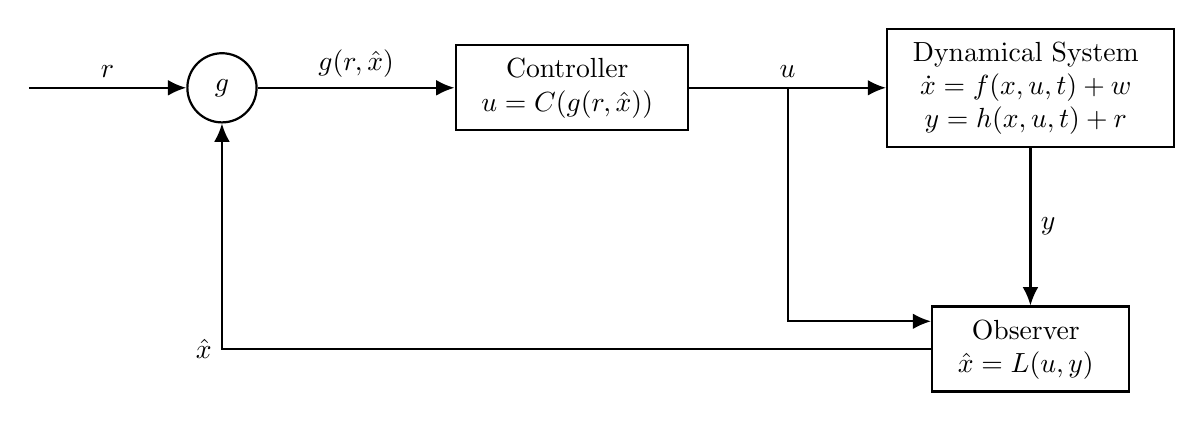
\begin{tikzpicture}[
  block/.style = {draw, thick, minimum height=3em, minimum width=6em, align=center},
  circ/.style  = {draw, circle, thick, minimum size=2.5em, inner sep=0pt},
  arrow/.style = {thick, -{Latex[width=2mm]}},
  node distance=2.5cm and 2.5cm
]

  % g node
  \node[circ] (g) {$g$};

  % Controller to the right of g
  \node[block, right=2.5cm of g] (controller) {
    \begin{tabular}{c}
      Controller \\
      $u = C(g(r,\hat{x}))$
    \end{tabular}
  };

  % System to the right of controller
  \node[block, right=2.5cm of controller] (system) {
    \begin{tabular}{c}
      Dynamical System \\
      $\dot{x} = f(x,u,t) + w$ \\
      $y = h(x,u,t) + r$
    \end{tabular}
  };

  % Observer below system
  \node[block, below=2cm of system] (observer) {
    \begin{tabular}{c}
      Observer \\
      $\hat{x} = L(u, y)$ 
    \end{tabular}
  };

  % r input
  \coordinate[left=2cm of g] (r_in);
  \draw[arrow] (r_in) -- node[above] {$r$} (g.west);

  % xhat from observer to g
  \draw[arrow] 
    (observer.west) -| (g.south)
    node[midway, left] {$\hat{x}$};

  % g(r,xhat) into controller
  \draw[arrow] (g.east) -- node[above] {$g(r,\hat{x})$} (controller.west);

  % u from controller to system
  \draw[arrow] (controller.east) -- node[above] {$u$} (system.west);

  % u elbow branch to observer
  \coordinate (usplit) at ($(controller.east)!0.5!(system.west)$);
  \coordinate[above=1em of observer.west] (observer_uin);
  \draw[arrow] (usplit) |- (observer_uin) node[pos=0.75, left] {};

  % y from system to observer
  \draw[arrow] (system.south) -- node[right] {$y$} (observer.north);

\end{tikzpicture}
\end{document}
